\chapter{TCP and Sockets: A Byte Stream, Not a Message Queue}\label{ch:tcp}

\begin{objectives}
\begin{itemize}
\item state TCP's service model precisely, including what it does \emph{not} promise;
\item walk the \cc{socket}/\cc{bind}/\cc{listen}/\cc{accept} lifecycle and say which kernel object each call creates;
\item explain the listen backlog and the two queues behind it;
\item prove that any protocol relying on \cc{recv} boundaries is incorrect, and reproduce the failure on loopback;
\item map each call onto \cc{Server::listen}, \cc{Connection}, and \cc{SocketHandle} in \texttt{score::net}.
\end{itemize}
{\small\color{muted}\textbf{Chapter references:} RFC 793 and RFC 9293~\cite{rfc793,rfc9293}; RFC 896~\cite{rfc896}; RFC 1122~\cite{rfc1122};
Stevens et al.~\cite{stevens2004unp}; Kerrisk~\cite{kerrisk2010tlpi}.}
\end{objectives}

\section{The service model}
TCP was specified in RFC~793 (1981)~\cite{rfc793} and consolidated in RFC~9293 (2022)~\cite{rfc9293}. Its promise to an
application is narrow, and most networking bugs come from assuming more than it gives.

\begin{definition}[Reliable byte stream]\label[definition]{def:bytestream}
A \emph{reliable byte stream} from $A$ to $B$ is a channel such that, if $A$ writes the byte sequences
$w_1, w_2, \dots, w_m$, then the concatenation of everything $B$ reads is a prefix of $w_1\Vert w_2\Vert\cdots\Vert w_m$,
and, absent failure, eventually the whole of it. Nothing is promised about how the bytes are grouped into reads.
\end{definition}

TCP provides two such streams per connection, one in each direction (full duplex). It handles loss, duplication and
reordering in the network with sequence numbers, acknowledgements and retransmission. It does \emph{not} carry the
application's write boundaries: a write is not a message, and a segment is not a write.

\begin{layman}
UDP is like posting letters: each envelope arrives whole or not at all, possibly out of order. TCP is like a garden
hose: the water arrives in order, but nobody can tell from the water where one bucketful ended and the next began. If
you need buckets, you have to mark them yourself. That marking is \emph{framing} (\cref{ch:framing}).
\end{layman}

\begin{proposition}[Boundary-blindness]\label[proposition]{prop:boundary}
Let $S=w_1\Vert\cdots\Vert w_m$ with $|S|=B$. Under \cref{def:bytestream}, any sequence of positive integers
$(\ell_1,\dots,\ell_q)$ with $\sum_j\ell_j=B$ is a permissible sequence of \cc{recv} return values (subject only to
each $\ell_j$ not exceeding the receiver's buffer size). Consequently an application protocol whose parsing depends on
the $\ell_j$ is not correct over TCP.
\end{proposition}
\begin{proof}
The definition constrains only the \emph{content} of the concatenated reads, never their lengths, so every
composition of $B$ is consistent with it. A protocol is correct only if it behaves correctly on every permitted
execution. If its output depends on $(\ell_j)$, two executions with equal byte content but different compositions give
different outputs, so at least one is wrong.
\end{proof}

The proposition is not hypothetical. \Cref{lst:streamdemo} writes one 44-byte frame (the one we will dissect in
\cref{ch:framing}) as three \cc{send} calls of 3, 20 and 21 bytes over loopback, with \cc{TCP_NODELAY} set, first with
50\,ms pauses and then with none.

\begin{code}{stream\_demo.cpp (excerpt): one frame, three writes}{lst:streamdemo}
const int cuts[] = {0, 3, 23, 44};
for (int i = 0; i < 3; ++i) {
    send(c, frame + cuts[i], cuts[i + 1] - cuts[i], 0);
    std::this_thread::sleep_for(std::chrono::milliseconds(pause_ms));
}
// ... server side, after accept():
for (ssize_t n; (n = recv(fd, buf, sizeof buf, 0)) > 0;) std::printf(" %zd", n);
\end{code}

\begin{progout}{stream\_demo on macOS loopback (two runs, identical)}{lst:streamout}
writes 3+20+21 with 50 ms pauses -> recv() returned: 3 20 21 0 (EOF)
writes 3+20+21 with 0 ms pauses -> recv() returned: 44 0 (EOF)
\end{progout}

The same bytes produced the read compositions $(3,20,21)$ and $(44)$ depending only on timing. A parser that
assumed ``one \cc{recv} = one request'' would see three garbage requests in the first run and be right only by luck in
the second. Over a real network, with a different maximum segment size, retransmissions and receive-window updates, the
compositions vary even more.

\section{The socket lifecycle}
A server needs a \emph{listening} socket, which never carries data, and one \emph{connected} socket per client.
\Cref{fig:tcp} shows the calls and the three-way handshake between them.

\begin{figure}[htbp]
\centering
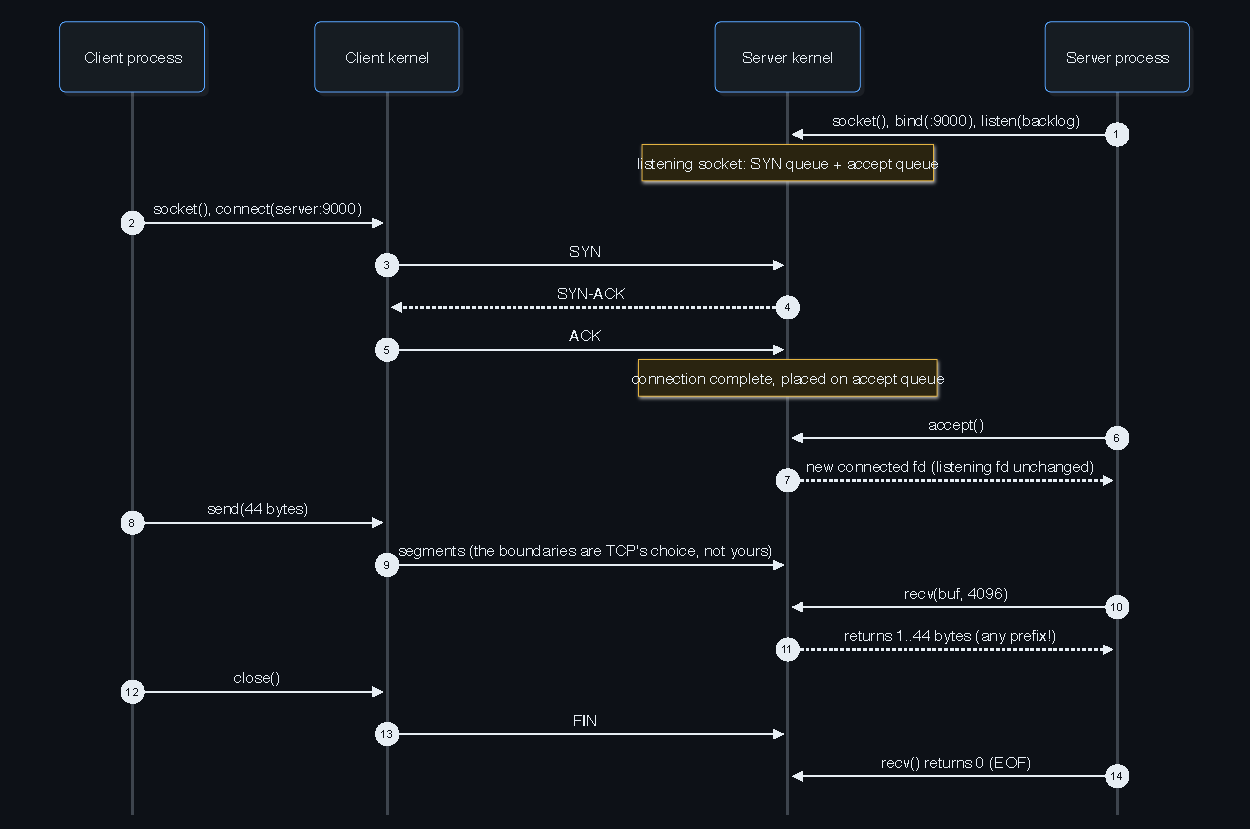
\includegraphics[width=\linewidth]{diagrams/tcp_lifecycle.pdf}
\caption{Server and client socket lifecycle, with the handshake performed by the kernels (Mermaid). The server process
is not involved in the handshake: \cc{accept} only dequeues a connection that the kernel has already completed.}
\label{fig:tcp}
\end{figure}

\begin{center}
\small
\begin{tabularx}{\linewidth}{@{}>{\leavevmode\ttfamily\color{org}}l X@{}}
\toprule
\textcolor{muted}{\rmfamily Call} & \textcolor{muted}{What it does in the kernel}\\
\midrule
socket(AF\_INET, SOCK\_STREAM, 0) & Allocates a socket object and returns a descriptor, a small integer indexing the process's file table. In \texttt{score} this is \cc{SocketHandle = int}.\\
setsockopt(SO\_REUSEADDR) & Allows \cc{bind} to an address with old connections still in TIME-WAIT, so a restarted server can rebind at once.\\
bind(fd, addr) & Attaches a local address and port.\\
listen(fd, backlog) & Marks the socket passive. The kernel now completes handshakes on its behalf and queues finished connections.\\
accept(fd) & Dequeues one completed connection and returns a \emph{new} descriptor for it. The listening descriptor is unchanged.\\
connect(fd, addr) & Client side: starts the handshake (SYN) and returns when it completes or fails.\\
recv / send & Copy bytes between user memory and the socket's kernel buffers. Either may move fewer bytes than asked.\\
shutdown(fd, SHUT\_WR) & Sends FIN (``I will write no more'') while still allowing reads: a half-close.\\
close(fd) & Releases the descriptor; the kernel finishes the connection teardown.\\
\bottomrule
\end{tabularx}
\end{center}

\subsection{The listen backlog}
The kernel holds two kinds of not-yet-accepted connections: those mid-handshake (SYN received, SYN-ACK sent) and those
complete but not yet returned by \cc{accept}. On Linux the \cc{backlog} argument bounds the second queue, the
\emph{accept queue}, and is silently capped by \cc{net.core.somaxconn}; half-open connections are governed separately by
\cc{tcp_max_syn_backlog}~\cite{kerrisk2010tlpi}. On the measurement machine, \cc{sysctl kern.ipc.somaxconn} reports
\texttt{128}. If the accept queue is full because the application is slow to call \cc{accept}, new clients see their SYNs
dropped or refused and retry with exponential back-off, which shows up as latency spikes of whole seconds rather than as
errors.

\begin{remarkbox}
The backlog is where the concurrency model of \cref{ch:conc} becomes visible to clients. A thread-per-connection server
calls \cc{accept} in a loop and hands off immediately, so its accept queue drains quickly until the machine runs out of
threads. A reactor calls \cc{accept} when the listening descriptor is reported \emph{readable}, so a slow handler on the
loop thread delays every \cc{accept}.
\end{remarkbox}

\section{Partial reads, partial writes, and the errors in between}
\Cref{prop:boundary} applies to writes too: \cc{send} on a non-blocking socket may accept fewer bytes than requested
when the kernel send buffer is nearly full, and then fails with \cc{EAGAIN} until space frees up. Correct code therefore
has the same shape on both sides:

\begin{code}{write\_all: the loop every sender needs (blocking socket)}{lst:writeall}
bool write_all(int fd, const std::uint8_t* p, std::size_t n) {
    while (n > 0) {
        ssize_t k = ::send(fd, p, n, 0);
        if (k < 0) {
            if (errno == EINTR) continue;   // interrupted by a signal: retry
            return false;                   // real error (EPIPE, ECONNRESET, ...)
        }
        p += k;                              // k may be < n: advance and loop
        n -= static_cast<std::size_t>(k);
    }
    return true;
}
\end{code}

On a non-blocking socket the reactor version cannot loop: on \cc{EAGAIN} it must keep the unsent tail in a per-connection
output buffer and register for \cc{IoEvent::kWritable}. That is precisely why \cc{Connection::send} is documented as
``\emph{queues} \cc{frame} for writing''.

\repo[firstline=9,lastline=29]{include/score/net/connection.hpp}{\cc{Connection} owns the descriptor and a codec and
holds a reference to the loop. The word ``queues'' in the comment on \cc{send} commits the implementation to an output
buffer, because a non-blocking write may be partial.}{lst:connection}

\subsection{Small writes and Nagle's algorithm}
Nagle's algorithm (RFC~896, 1984)~\cite{rfc896} holds back a small segment while earlier data is unacknowledged, and
receivers commonly delay ACKs~\cite{rfc1122}. A sender that writes a 4-byte length prefix and then the payload as
\emph{two} writes can stall for a delayed-ACK interval waiting for an acknowledgement. Two habits avoid it:
build the whole frame in one buffer (as \cc{FrameCodec::encode} does by returning a single \cc{std::vector<std::uint8_t>}),
or use a gather write (\cc{writev}). Setting \cc{TCP_NODELAY} disables Nagle's algorithm but does not make two writes
one.

\section{Mapping onto \texttt{score::net}}
\repo[firstline=13,lastline=38]{include/score/net/server.hpp}{\cc{Server::listen(port)} will be
\cc{socket}+\cc{setsockopt}+\cc{bind}+\cc{listen}, then registration of the listening descriptor with the loop for
readability. Each readable event on it means ``\cc{accept} will not block''. Each accepted descriptor gets a fresh codec
from \cc{CodecFactory}, because codecs hold per-connection buffers.}{lst:server}

\begin{example}[One request, end to end]\label[example]{ex:e2e}
A pre-trade client connects, writes the 44-byte frame of \cref{fig:frame} and waits. The server kernel completes the
handshake and queues the connection; the loop reports the listening descriptor readable; \cc{Server} calls \cc{accept}
and creates a \cc{Connection} with a new \cc{JsonFrameCodec}; the loop later reports the connection readable; the
callback \cc{recv}s some prefix of the 44 bytes and \cc{feed}s it to the codec; \cc{try_decode} returns \cc{nullopt}
until all 44 bytes have arrived (\cref{thm:segmentation}); the handler computes VaR and \cc{send}s a reply frame, which
may itself take several writes.
\end{example}

\begin{exercises}
\ex{ex:listen}{\lvA} Write the exact sequence of system calls \cc{Server::listen(9000)} should make, including
\cc{SO_REUSEADDR}, \cc{O_NONBLOCK} and the loop registration. Say what goes wrong in a test suite that restarts the
server on the same port if \cc{SO_REUSEADDR} is omitted.

\ex{ex:compositions}{\lvB} A client sends two 44-byte frames back to back. How many distinct \cc{recv} return sequences
are possible if the server's buffer is 64 bytes? Which of them leave the second frame's length prefix split across two
reads? (Count compositions with bounded parts.)

\ex{ex:sendq}{\lvB} \cc{Connection::send} is called from a request handler while the kernel send buffer is full. Design the
output queue: data structure, when to register and unregister \cc{kWritable}, and a cap that stops a slow reader from
exhausting server memory. What should happen to the connection when the cap is hit?

\ex{ex:backlog}{\lvC} With the accept queue full, what exactly does a client observe on Linux, and what on macOS?
Design an experiment with a server that never calls \cc{accept}, and predict the client's \cc{connect} latency
distribution before running it.

\ex{ex:halfclose}{\lvB} A backtest client sends 500 requests and then has nothing more to say, but still needs the 500
replies. Explain how \cc{shutdown(SHUT_WR)} helps the server, and what the server's read loop sees.
\end{exercises}

